\section{The \fermi Gamma-ray Space Telescope}

\begin{figure}[htbp]
  \centering
    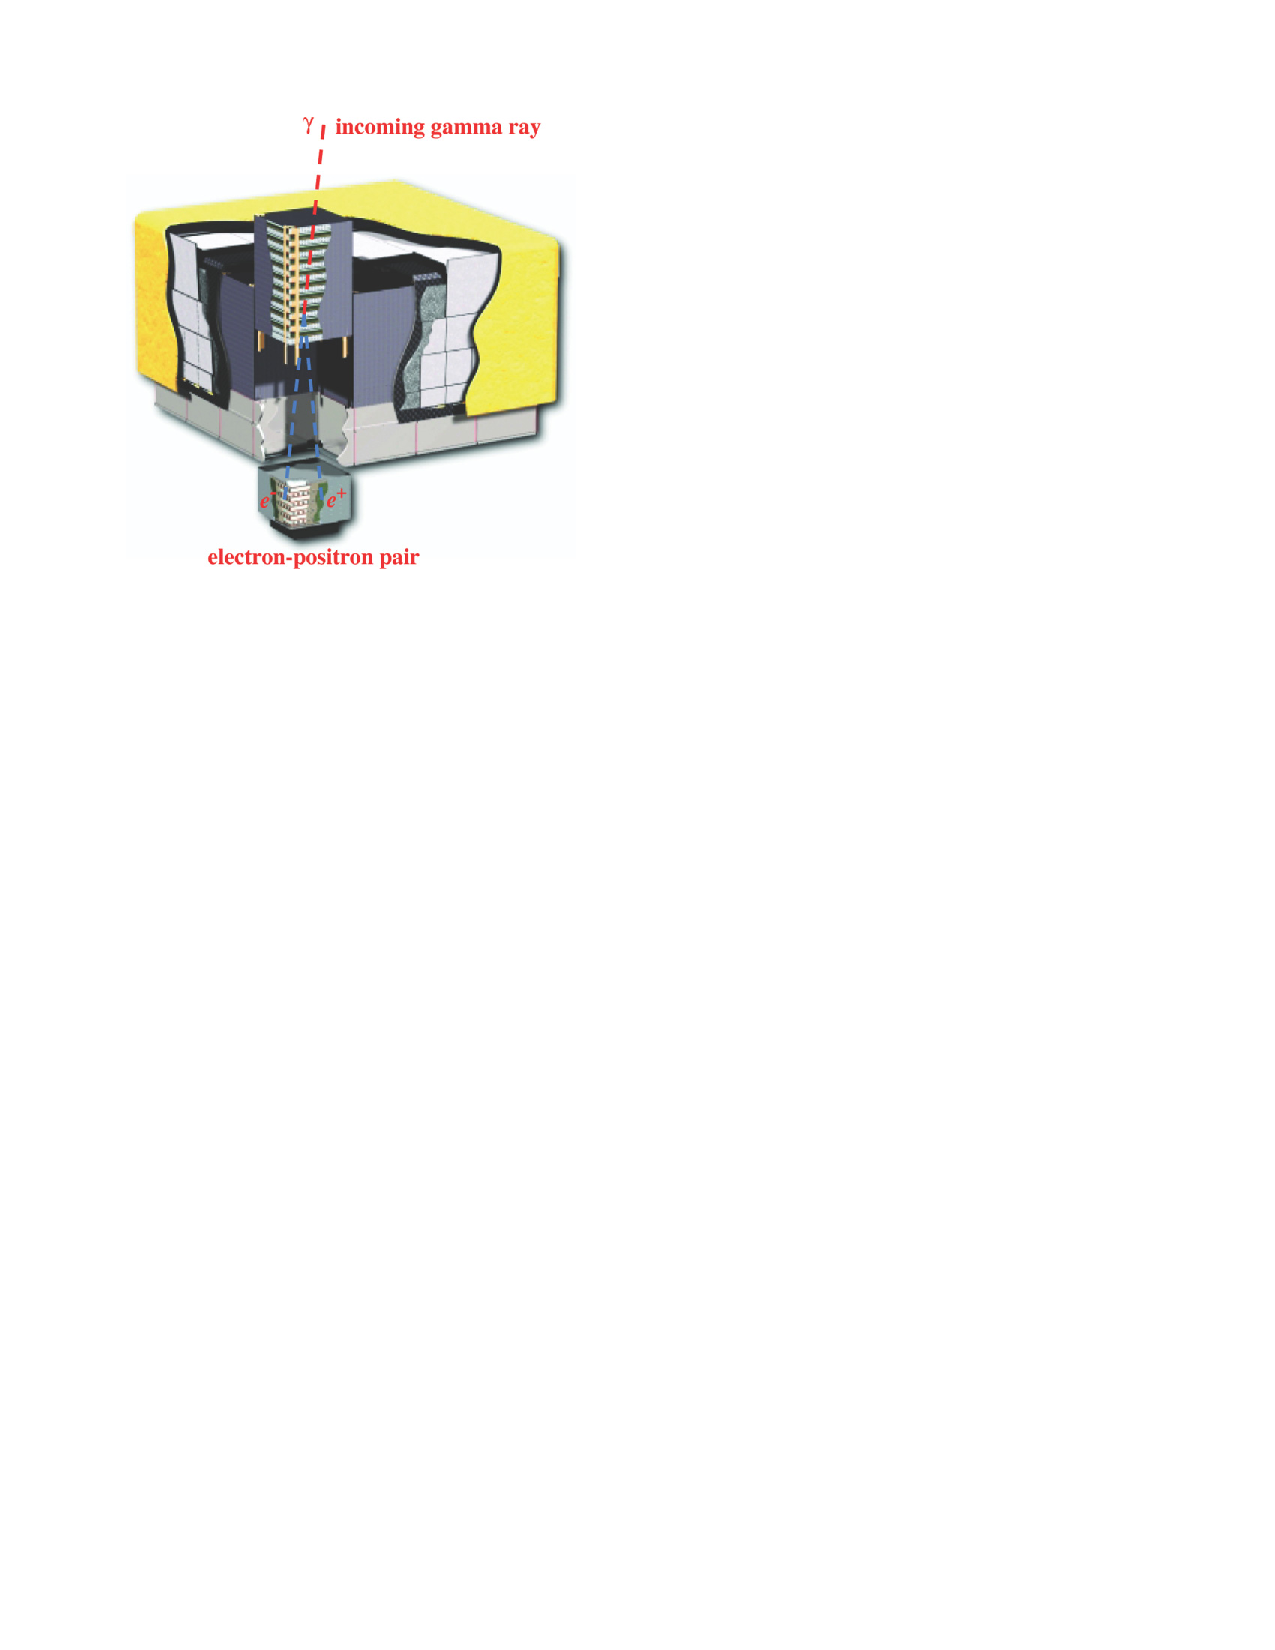
\includegraphics{chapters/introduction/figures/lat_detector_cutout.pdf}
  \caption{A schematic diagram of the \ac{LAT} with an incident $\gamma$-ray
    (red line) pair-converting into an electron and positron (blue lines)
    which are recorded in the tracker and calorimiter of the \ac{LAT}.
    This figure is taken from \citep{atwood_2009a_large-telescope}.  
  }
  \figlabel{lat_detector_cutout}
\end{figure} 


the \fermi Gamma-ray Space telescope was launched on June 11, 2008 on
a Delta II Heavy laucnh vehicle \citep{atwood_2009a_large-telescope}.
The primary since instrument on board \fermi is the \ac{LAT},
which is a pair-conversion telescope which detects $\gamma$-rays in
the energy range from $20\unitspace\mev$ to $>300\unitspace\gev$.
\figref{lat_detector_cutout} shows a schematic diagram of the \ac{LAT}.


With its $2.4\unitspace\steradian$ filed of view,


is a pair-conversion detector which measures 

The \Ac{LAT} on board 

\subsection{The Tracker}
\subsection{The Calorimiter}
\subsection{\Acl{ACD}}

The \Ac{ACD} is \ldots

\subsection{\Acl{GBM}}

\seclabel{fermi_telescope}

\subsection{Performance of the \acs{LAT}}
